\documentclass[glossy]{beamer}
\useoutertheme{wuerzburg}
\useinnertheme[realshadow,corners=2pt,padding=2pt]{chamfered}
\usecolortheme{shark}

\usepackage{listings}
\usepackage[utf8]{inputenc}


\usepackage{fancyvrb}
%\usepackage[scaled]{beramono} %sets the beramono font. Just comment this line to get the default font back

\usepackage{tikz}
\newcommand<>{\hover}[1]{\uncover#2{%
 \begin{tikzpicture}[remember picture,overlay]%
 \draw[fill,opacity=0.4] (current page.south west)
 rectangle (current page.north east);
 \node at (current page.center) {#1};
 \end{tikzpicture}}
}

\title{Arquitecturas y Organización de Computadoras I \\\line(1,0){320}}
% \author{\texorpdfstring{Author\newline\url{email@email.com}}{Author}}
%\author{Rafael Ignacio Zurita}
\institute{Rafael Ignacio Zurita \\ Departamento de Ingenieria de Computadoras - FAI - UNCOMA 2018 \\ Clase presencial 5}
%\date{\today}



\begin{document}




\begin{frame}
\maketitle
\end{frame}

\institute{Departamento de Ingenieria de Computadoras - FAI - UNCOMA \\ 2018}

\begin{frame}
\frametitle{Programa Analítico}
\textbf{UNIDAD 2: Unidad Central de Proceso}
 \\~\\
Introducción al diseño lógico. Tablas de verdad. Álgebra de Boole.  Circuitos  combinacionales.  Relojes.  Elementos  de memoria.  Flip-flops,  cerrojos (latches) .  Circuitos  secuenciales.  Implementación de FSM. Circuitos lógicos programables. Unidad Lógica aritmética. Implementación de la suma, resta y operaciones lógicas.  Concepto  de  máquinas  algorítmicas.  Camino  de  datos.  Unidad  de  control.  Implementación  del  algoritmo    básico  de multiplicación. Conceptos de representación de número en punto flotante y error. Suma y multiplicación de punto flotante.
 \\~\\
\end{frame}


\begin{frame}
\frametitle{Temario}
\begin{itemize}
\item Operaciones (instrucciones) y el conjunto de instrucciones MIPS
\item Modos de direccionamiento
\item Lenguaje Máquina
\item Ensamblador
\item Traducción de declaraciones en C a lenguaje ensamblador
\end{itemize}
\end{frame}


\begin{frame}
\frametitle{Compuertas, Tablas de Verdad, Ecuaciones Lógicas}
\begin{center}\textbf{Señales digitales}\end{center}
\begin{itemize}
\item La electrónica interna de un computador actual 
es digital
\item La electrónica digital opera con dos niveles de 
voltaje: un voltaje alto y un voltaje bajo
\item El resto de los valores de voltaje son 
temporales y ocurren durante la transición 
entre los valores alto y bajo o bajo y alto
\end{itemize}
\end{frame}







\begin{frame}
\frametitle{Compuertas, Tablas de Verdad, Ecuaciones Lógicas}
\begin{center}\textbf{Señales digitales}\end{center}
\begin{itemize}
\item Esta es una razón clave por la que los 
computadores utilizan números binarios, ya 
que un sistema binario se corresponde 
directamente con la abstracción subyacente a 
la electrónica
\item En las diferentes implementaciones 
electrónicas los voltajes y sus relaciones difieren,
\item Por lo que no se utiliza el valor del voltage sino una indicación de si la señal esta activada o no (verdadera o no, 1 o 0, etc).

\end{itemize}
\end{frame}





\begin{frame}
\frametitle{Compuertas, Tablas de Verdad, Ecuaciones Lógicas}
\begin{center}\textbf{Señales digitales}\end{center}
\begin{itemize}
\item Por eso hablamos de señales que son:
\begin{itemize}
\item (lógicamente) ciertas, ó 1, ó 
afirmadas, asertadas
\item (lógicamente) falsas, ó 0, ó  
negadas
\end{itemize}
\item Los valores 0 y 1 reciben el nombre de 
complementarios o inversos
 el uno del otro

\end{itemize}
\end{frame}



\begin{frame}
\frametitle{Compuertas, Tablas de Verdad, Ecuaciones Lógicas}
\begin{center}\textbf{Diseño digital}\end{center}
\begin{itemize}
\item Los bloques lógicos 
(circuitos digitales o lógicos)
 se 
clasifican en dos tipos:
\begin{itemize}
\item circuitos combinacionales
\begin{itemize}
\item Sus salidas dependen sólo de las entradas
\end{itemize}
\item circuitos secuenciales

\begin{itemize}
\item Mantienen un estado interno. Sus salidas pueden 
depender tanto de las entradas actuales como
del valor almacenado en memoria, conocido 
como estado del bloque
\end{itemize}

\end{itemize}
\end{itemize}
\end{frame}





\begin{frame}
\frametitle{Compuertas, Tablas de Verdad, Ecuaciones Lógicas}
\begin{center}\textbf{Tablas de Verdad}\end{center}
\begin{itemize}
\item Debido a que un bloque de lógica combinatoria 
no contiene memoria, puede especificarse 
completamente definiendo los valores de las 
salidas para cada posible conjunto de valores 
de entrada
\item 
Dicha descripción se da normalmente en forma 
de 
tabla de verdad

\end{itemize}
\end{frame}




\begin{frame}
\frametitle{Compuertas, Tablas de Verdad, Ecuaciones Lógicas}
\begin{center}\textbf{Tablas de Verdad}\end{center}
\begin{itemize}
\item Para un bloque lógico con n entradas, existen   2 n posiciones en la tabla de verdad, puesto que 
este es el número de combinaciones posible de 
los valores de entrada
\item Cada posición en la tabla especifica el valor de 
todas las salidas para una combinación 
particular de las entrada
\item Las tablas de verdad pueden \textbf{describir 
completamente cualquier función lógica} 
combinatoria
\item Sin embargo, su tamaño \textbf{crece rápidamente} y 
puede dificultar su comprensión

\end{itemize}
\end{frame}


%\begin{frame}
%\frametitle{Compuertas, Tablas de Verdad, Ecuaciones Lógicas}
%\begin{center}\textbf{Tablas de Verdad}\end{center}
%\begin{figure}
%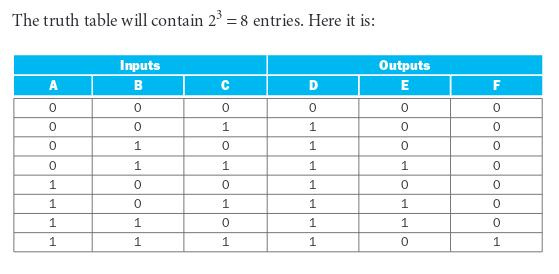
\includegraphics[scale=0.4]{tabla.jpg} 
%\end{figure}
%
%
%\end{frame}











\begin{frame}
\frametitle{Compuertas, Tablas de Verdad, Ecuaciones Lógicas}
\begin{center}\textbf{Algebra de Boole}\end{center}
\begin{itemize}
\item Todas la variable tienen valores 0 ó 1
\item Existen tres operadores:
\begin{itemize}
\item \textbf{OR}
, se escribe 
+
, como en 
A +B
. El resultado es 1 si alguna 
de la variables de entrada es 1. También se conoce como 
suma lógica
\item \textbf{AND}
, se escribe
 .
, como en
 A.B
. El resultado es 1 sólo si 
ambas entradas son 1. También se conoce como 
producto 
lógico
\item \textbf{NOT}
, se escribe      . El resultado es 1 sólo si la entrada es 0. 
La aplicación del operador NOT a un valor lógico resulta en 
una inversión o negación de dicho valor 
\end{itemize}
\end{itemize}
\end{frame}






\begin{frame}
\frametitle{Compuertas, Tablas de Verdad, Ecuaciones Lógicas}
\begin{center}\textbf{Álgebra de Boole - Leyes y Teoremas}\end{center}
\begin{figure}
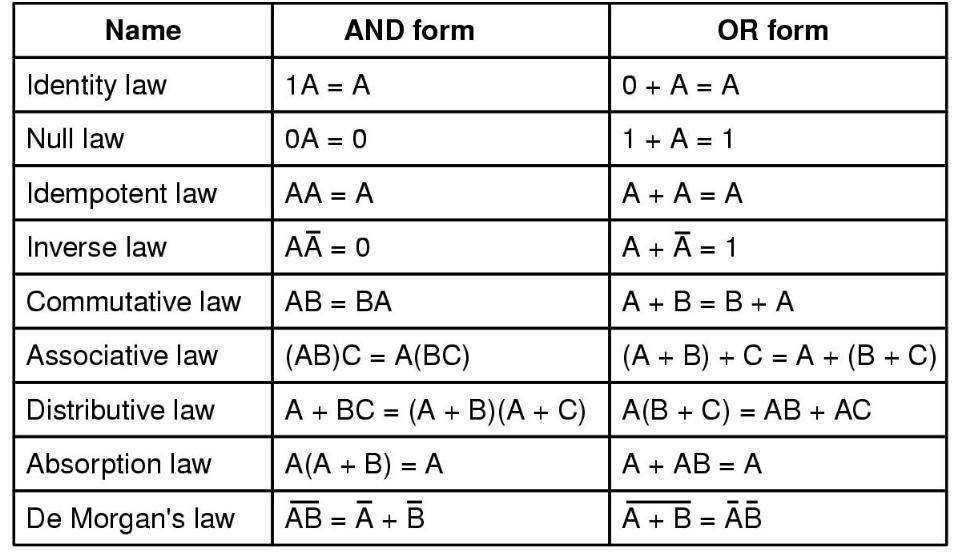
\includegraphics[scale=0.2]{leyes.jpg} 
\end{figure}
\end{frame}







\begin{frame}
\frametitle{Compuertas, Tablas de Verdad, Ecuaciones Lógicas}
\begin{center}\textbf{Álgebra de Boole - Leyes y Teoremas}\end{center}
\begin{itemize}
\item Cualquier función lógica puede ser reescrita como una ecuación, 
con la salida en la parte izquierda de la igualdad, y una función 
de las variables de entrada utilizando las operaciones del álgebra a la derecha.

\item Ejemplo:
\end{itemize}
\begin{figure}
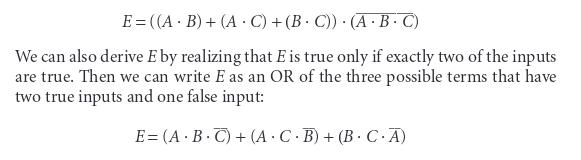
\includegraphics[scale=0.4]{ecuacion.jpg} 
\end{figure}
\end{frame}




\begin{frame}[fragile]
\frametitle{Diseño digital}
\begin{center}\textbf{Compuertas/Puertas (Gates)}\end{center}
\begin{itemize}
\item Los bloques lógicos se construyen a partir de 
compuertas (puertas) lógicas
 que realizan las 
funciones lógicas básicas como AND, OR y NOT
\item Una puerta AND o una OR pueden tener 
múltiples entradas, con la salida igual a la AND o 
la OR de todas ellas
\item La función lógica NOT se realiza mediante un 
inversor que siempre tiene una entrada
\end{itemize}

\end{frame}





\begin{frame}[fragile]
\frametitle{Diseño digital}
\begin{center}\textbf{Compuertas/Puertas (Gates)}\end{center}
\begin{figure}
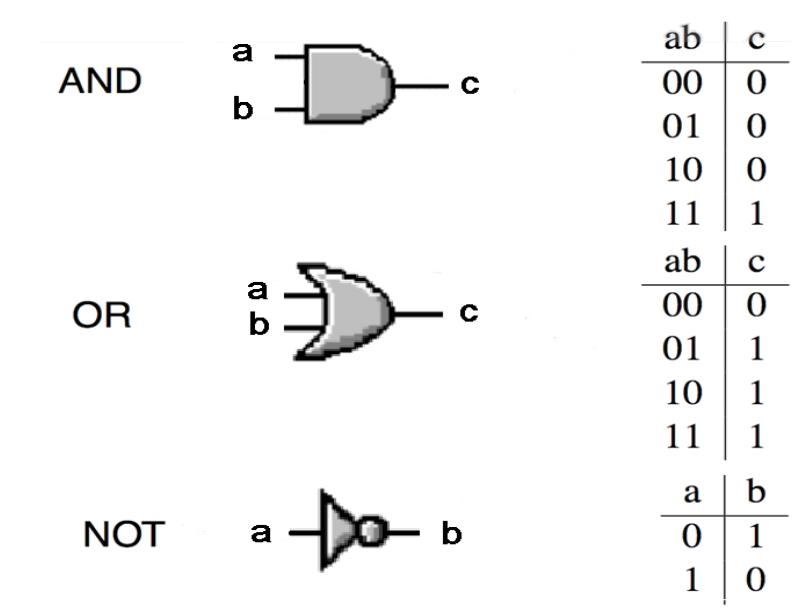
\includegraphics[scale=0.2]{compuertas.jpg} 
\end{figure}
\end{frame}


\begin{frame}[fragile]
\frametitle{Diseño digital}
\begin{center}\textbf{Compuertas/Puertas (Gates)}\end{center}
\begin{figure}
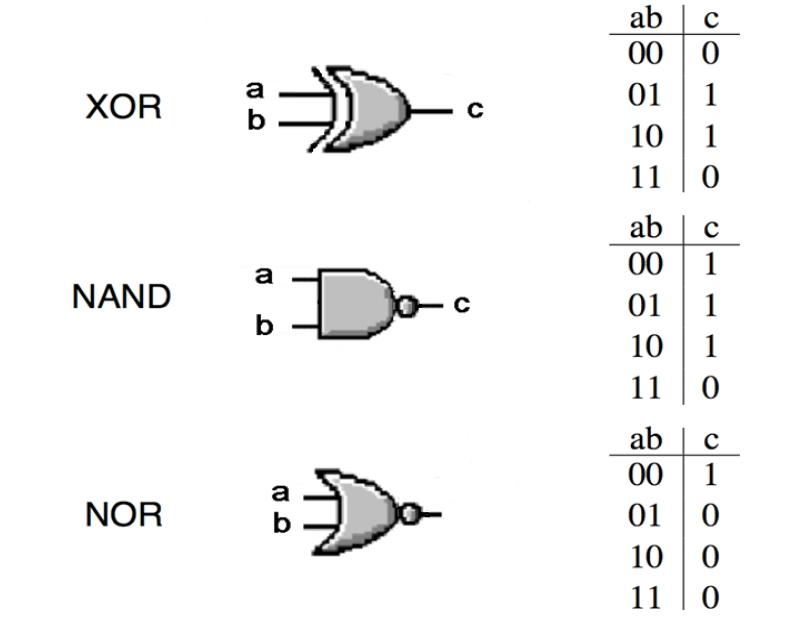
\includegraphics[scale=0.2]{compuertasx.jpg} 
\end{figure}
\end{frame}


\begin{frame}[fragile]
\frametitle{Diseño digital}
\begin{center}\textbf{Construcción de diseño lógico/digital}\end{center}
\begin{figure}
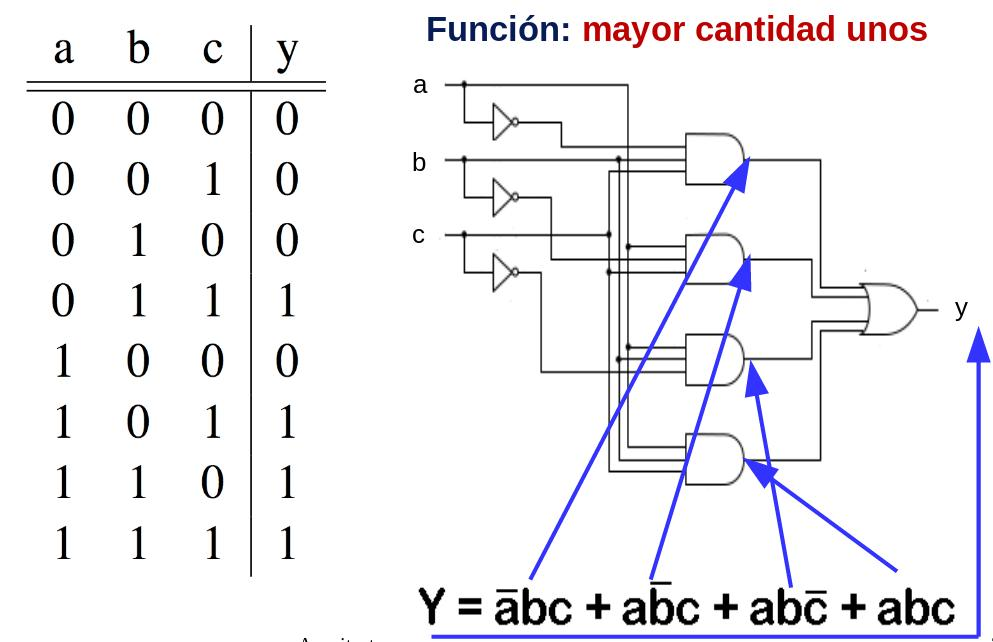
\includegraphics[scale=0.2]{construcciondigital.jpg} 
\end{figure}
\end{frame}




\begin{frame}[fragile]
\frametitle{Diseño digital}
\begin{center}\textbf{Construcción de diseño lógico/digital: Decoder}\end{center}
\begin{figure}
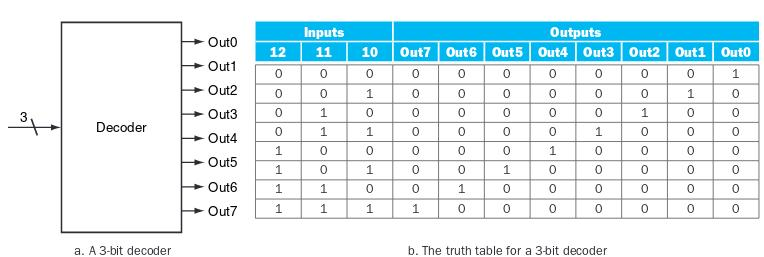
\includegraphics[scale=0.4]{decoder.jpg} 
\end{figure}
\end{frame}


\begin{frame}[fragile]
\frametitle{Diseño digital}
\begin{center}\textbf{Construcción de diseño lógico/digital: Multiplexor}\end{center}
\begin{figure}
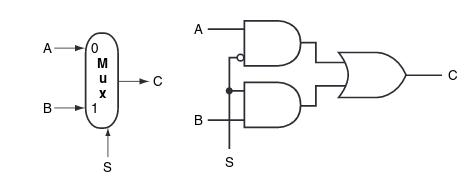
\includegraphics[scale=0.4]{multiplexor.jpg} 
\end{figure}
\end{frame}



\begin{frame}[fragile]
\frametitle{Diseño digital}
\begin{center}\textbf{Construcción de diseño lógico/digital: Multiplexor 32 bits}\end{center}
\begin{figure}
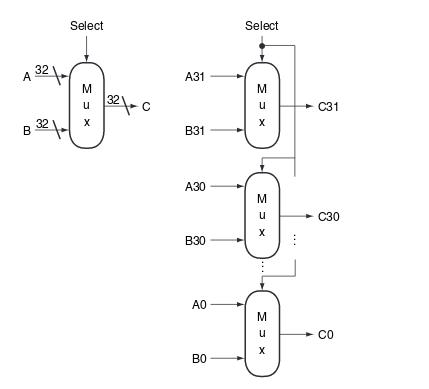
\includegraphics[scale=0.4]{multiplexor32bits.jpg} 
\end{figure}
\end{frame}




\begin{frame}[fragile]
\frametitle{Diseño digital}
\begin{center}\textbf{Diseño de ALU de un bit}\end{center}
\begin{figure}
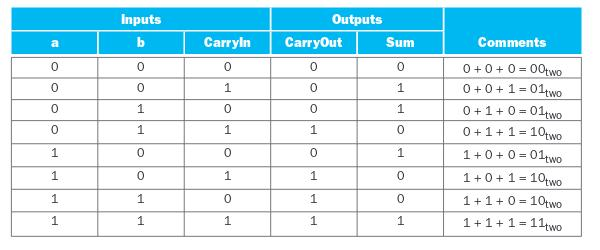
\includegraphics[scale=0.4]{alu1bit.jpg} 
\end{figure}
\end{frame}




\begin{frame}[fragile]
\frametitle{Diseño digital}
\begin{center}\textbf{Diseño de ALU de un bit}\end{center}
\begin{figure}
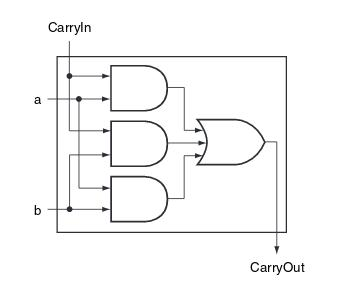
\includegraphics[scale=0.4]{alu1bit-2.jpg} 
\end{figure}
\end{frame}




\begin{frame}[fragile]
\frametitle{Diseño digital}
\begin{center}\textbf{Diseño de ALU de un bit}\end{center}
\begin{figure}
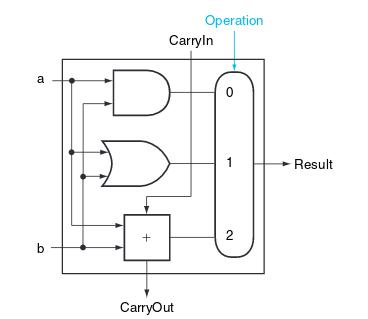
\includegraphics[scale=0.4]{alu1bit-3.jpg} 
\end{figure}
\end{frame}


\begin{frame}[fragile]
\frametitle{Diseño digital}
\begin{center}\textbf{Diseño de ALU de un bit}\end{center}
\begin{figure}
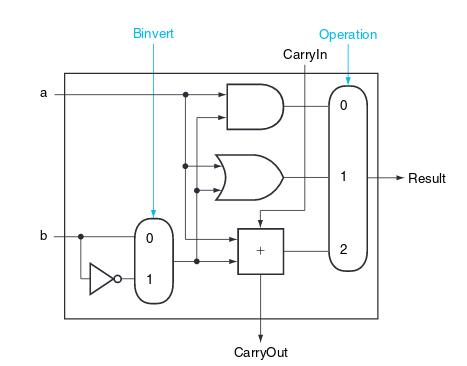
\includegraphics[scale=0.4]{alu1bit-4.jpg} 
\end{figure}
\end{frame}


\begin{frame}[fragile]
\frametitle{Diseño digital}
\begin{center}\textbf{Diseño de ALU de 32 bits}\end{center}
\begin{figure}
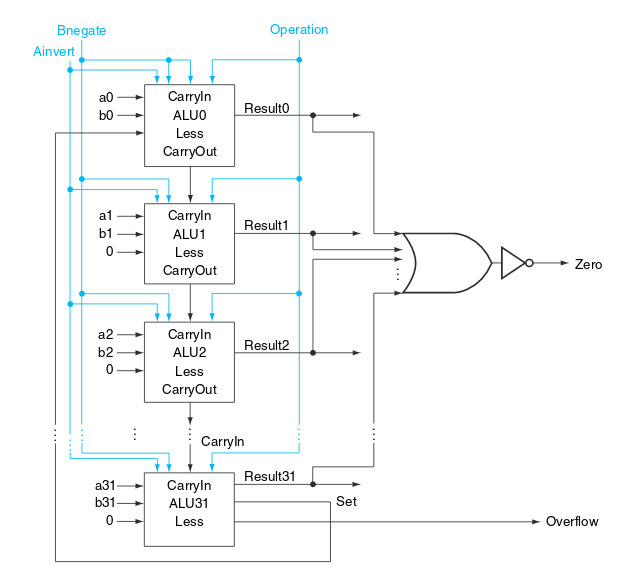
\includegraphics[scale=0.4]{alu1bit-5.jpg} 
\end{figure}
\end{frame}


\begin{frame}[fragile]
\frametitle{Diseño digital}
\begin{center}\textbf{Diseño de una unidad de control}\end{center}
\begin{figure}
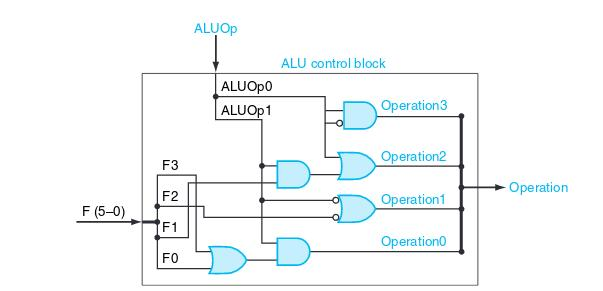
\includegraphics[scale=0.4]{control.jpg} 
\end{figure}
\end{frame}





\begin{frame}
 \frametitle{Consejos y preguntas}
\begin{center}
\begin{itemize}
\item  ¿Preguntas?
\end{itemize}
\end{center}
\end{frame}


\begin{frame}
 \frametitle{Bibliografía}
Libros
\begin{itemize}
\item Andrew S. Tanenbaum (2000), ORGANIZACIÓN DE COMPUTADORAS un enfoque estructurado, Editorial Prentice Hall. (10 copias en biblioteca)
\item David. Patterson John L. Hennessy (1995), ORGANIZACIÓN Y DISEÑO DE COMPUTADORES La interfaz hardware/software, McGraw-Hill (8 copias en biblioteca).
\end{itemize}
Contenido electrónico
\begin{itemize}
	\item \textbf{x86 assembly basis} Una introducción al lenguaje ensamblador x86. Disponible en PEDCO en formato PDF.
		\url{https://www.nayuki.io/page/a-fundamental-introduction-to-x86-assembly-programming}
\item Apuntes elaborados por la cátedra, disponibles en PEDCO para impresión (pdf) o lectura online (html)
\item Secciones de libros aptas para publicacion
\end{itemize}
\end{frame}


\end{document}
